% !TeX encoding = UTF-8
% !TeX program  = pdflatex

\documentclass[xcolor={svgnames,table},10pt,fleqn]{beamer}
\usepackage{stb-beamer-a}

%---- AMS math ---------------------------------------------------------
\usepackage{amsmath,amsthm}

%---- Fonts ------------------------------------------------------------
\usefonttheme{professionalfonts}
\usepackage[T1]{fontenc}
\usepackage{textcomp}
\usepackage[default,medium,scaled=1.0]{raleway}
\usepackage[scaled=0.80]{arevmath}

%---- Packages ---------------------------------------------------------
\usepackage{tikz}
\usepackage{booktabs}
\cmidrulewidth=\heavyrulewidth

\graphicspath{{imgs/}}

%---- Title page -------------------------------------------------------
\title[\emph{Ergo}]{\emph{Ergo}}
\subtitle{A Gesture-Based Computer Interaction Device}

\author{Boyd Kane, Supervisor: Dr. Trienko Grobler}
\institute{Computer Science Division,\\
           Stellenbosch University}

\subject{Master's in Computer Science}
\date{February 2024}

\def\titlefig{{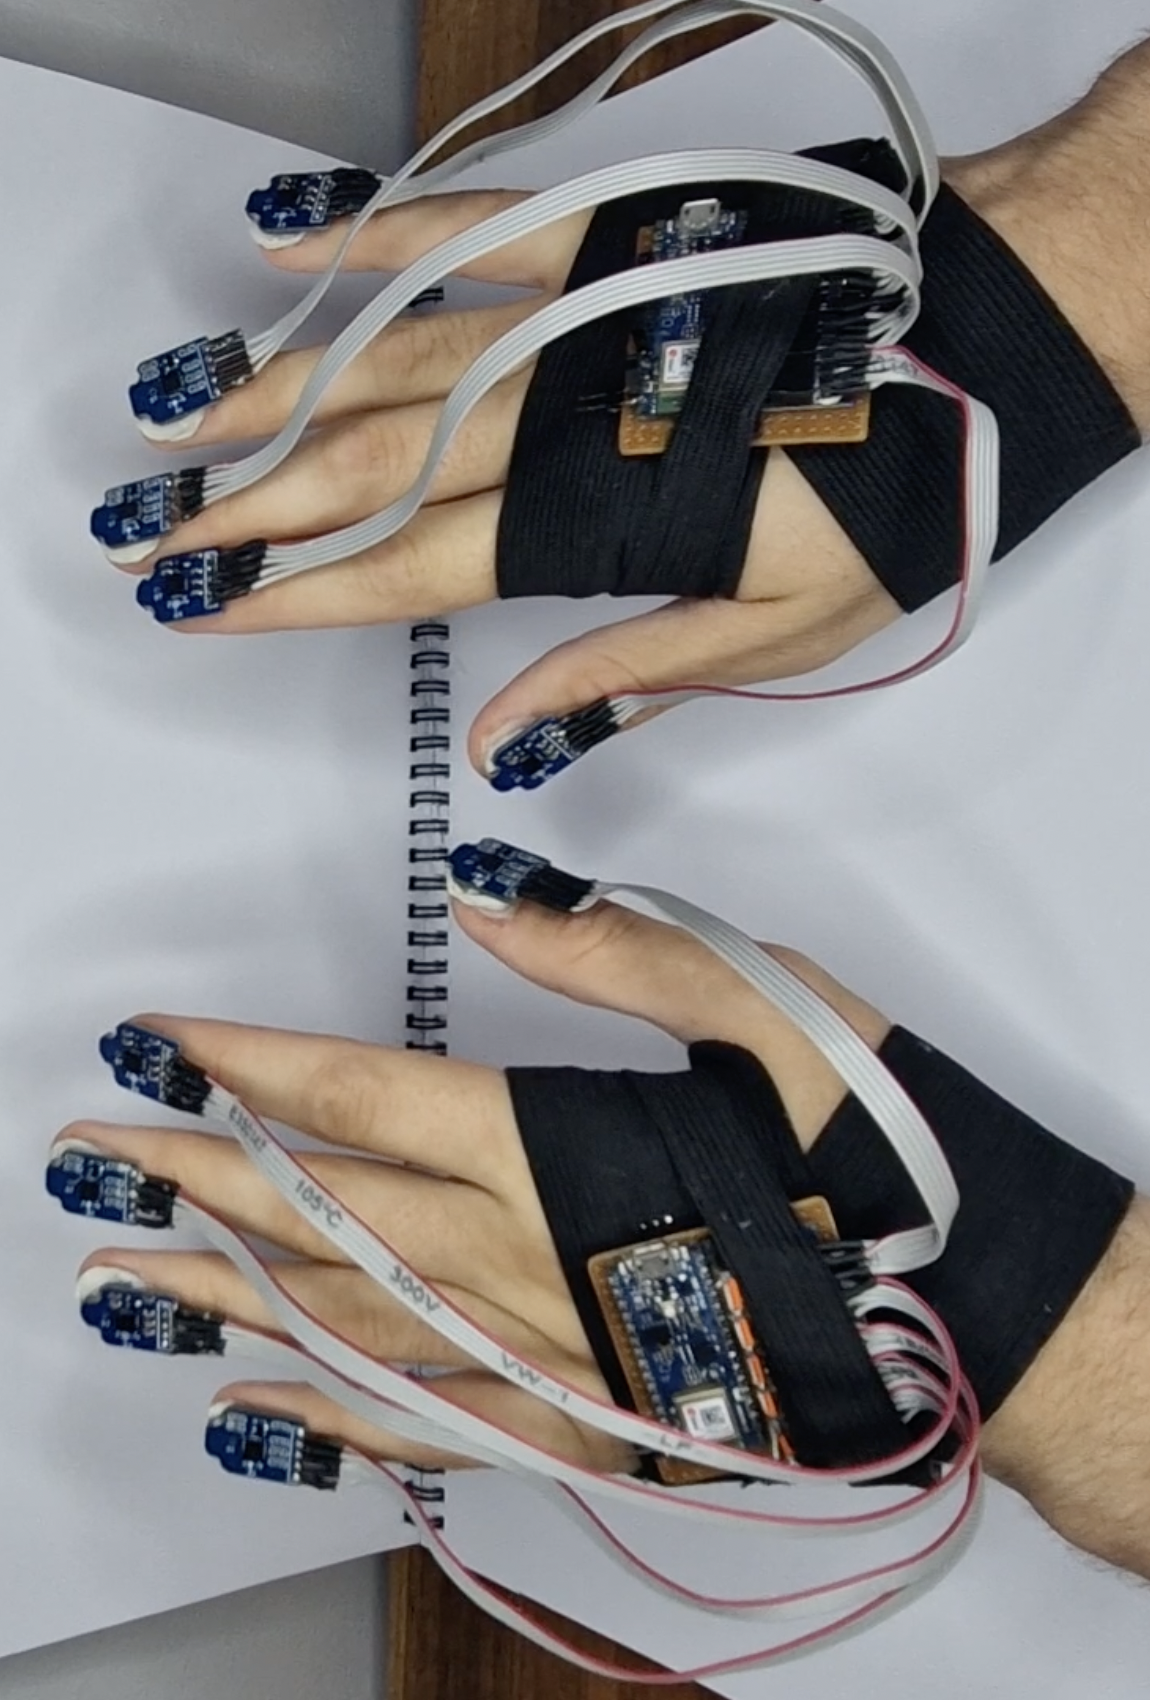
\includegraphics[height=5.5cm, angle=270]{glove}}}

\begin{document}
\begin{frame}
  \maketitle
\end{frame}

\section{Overview}
\begin{frame}
    \frametitle{A video demonstration}
    \begin{figure}[h]
        \centering
        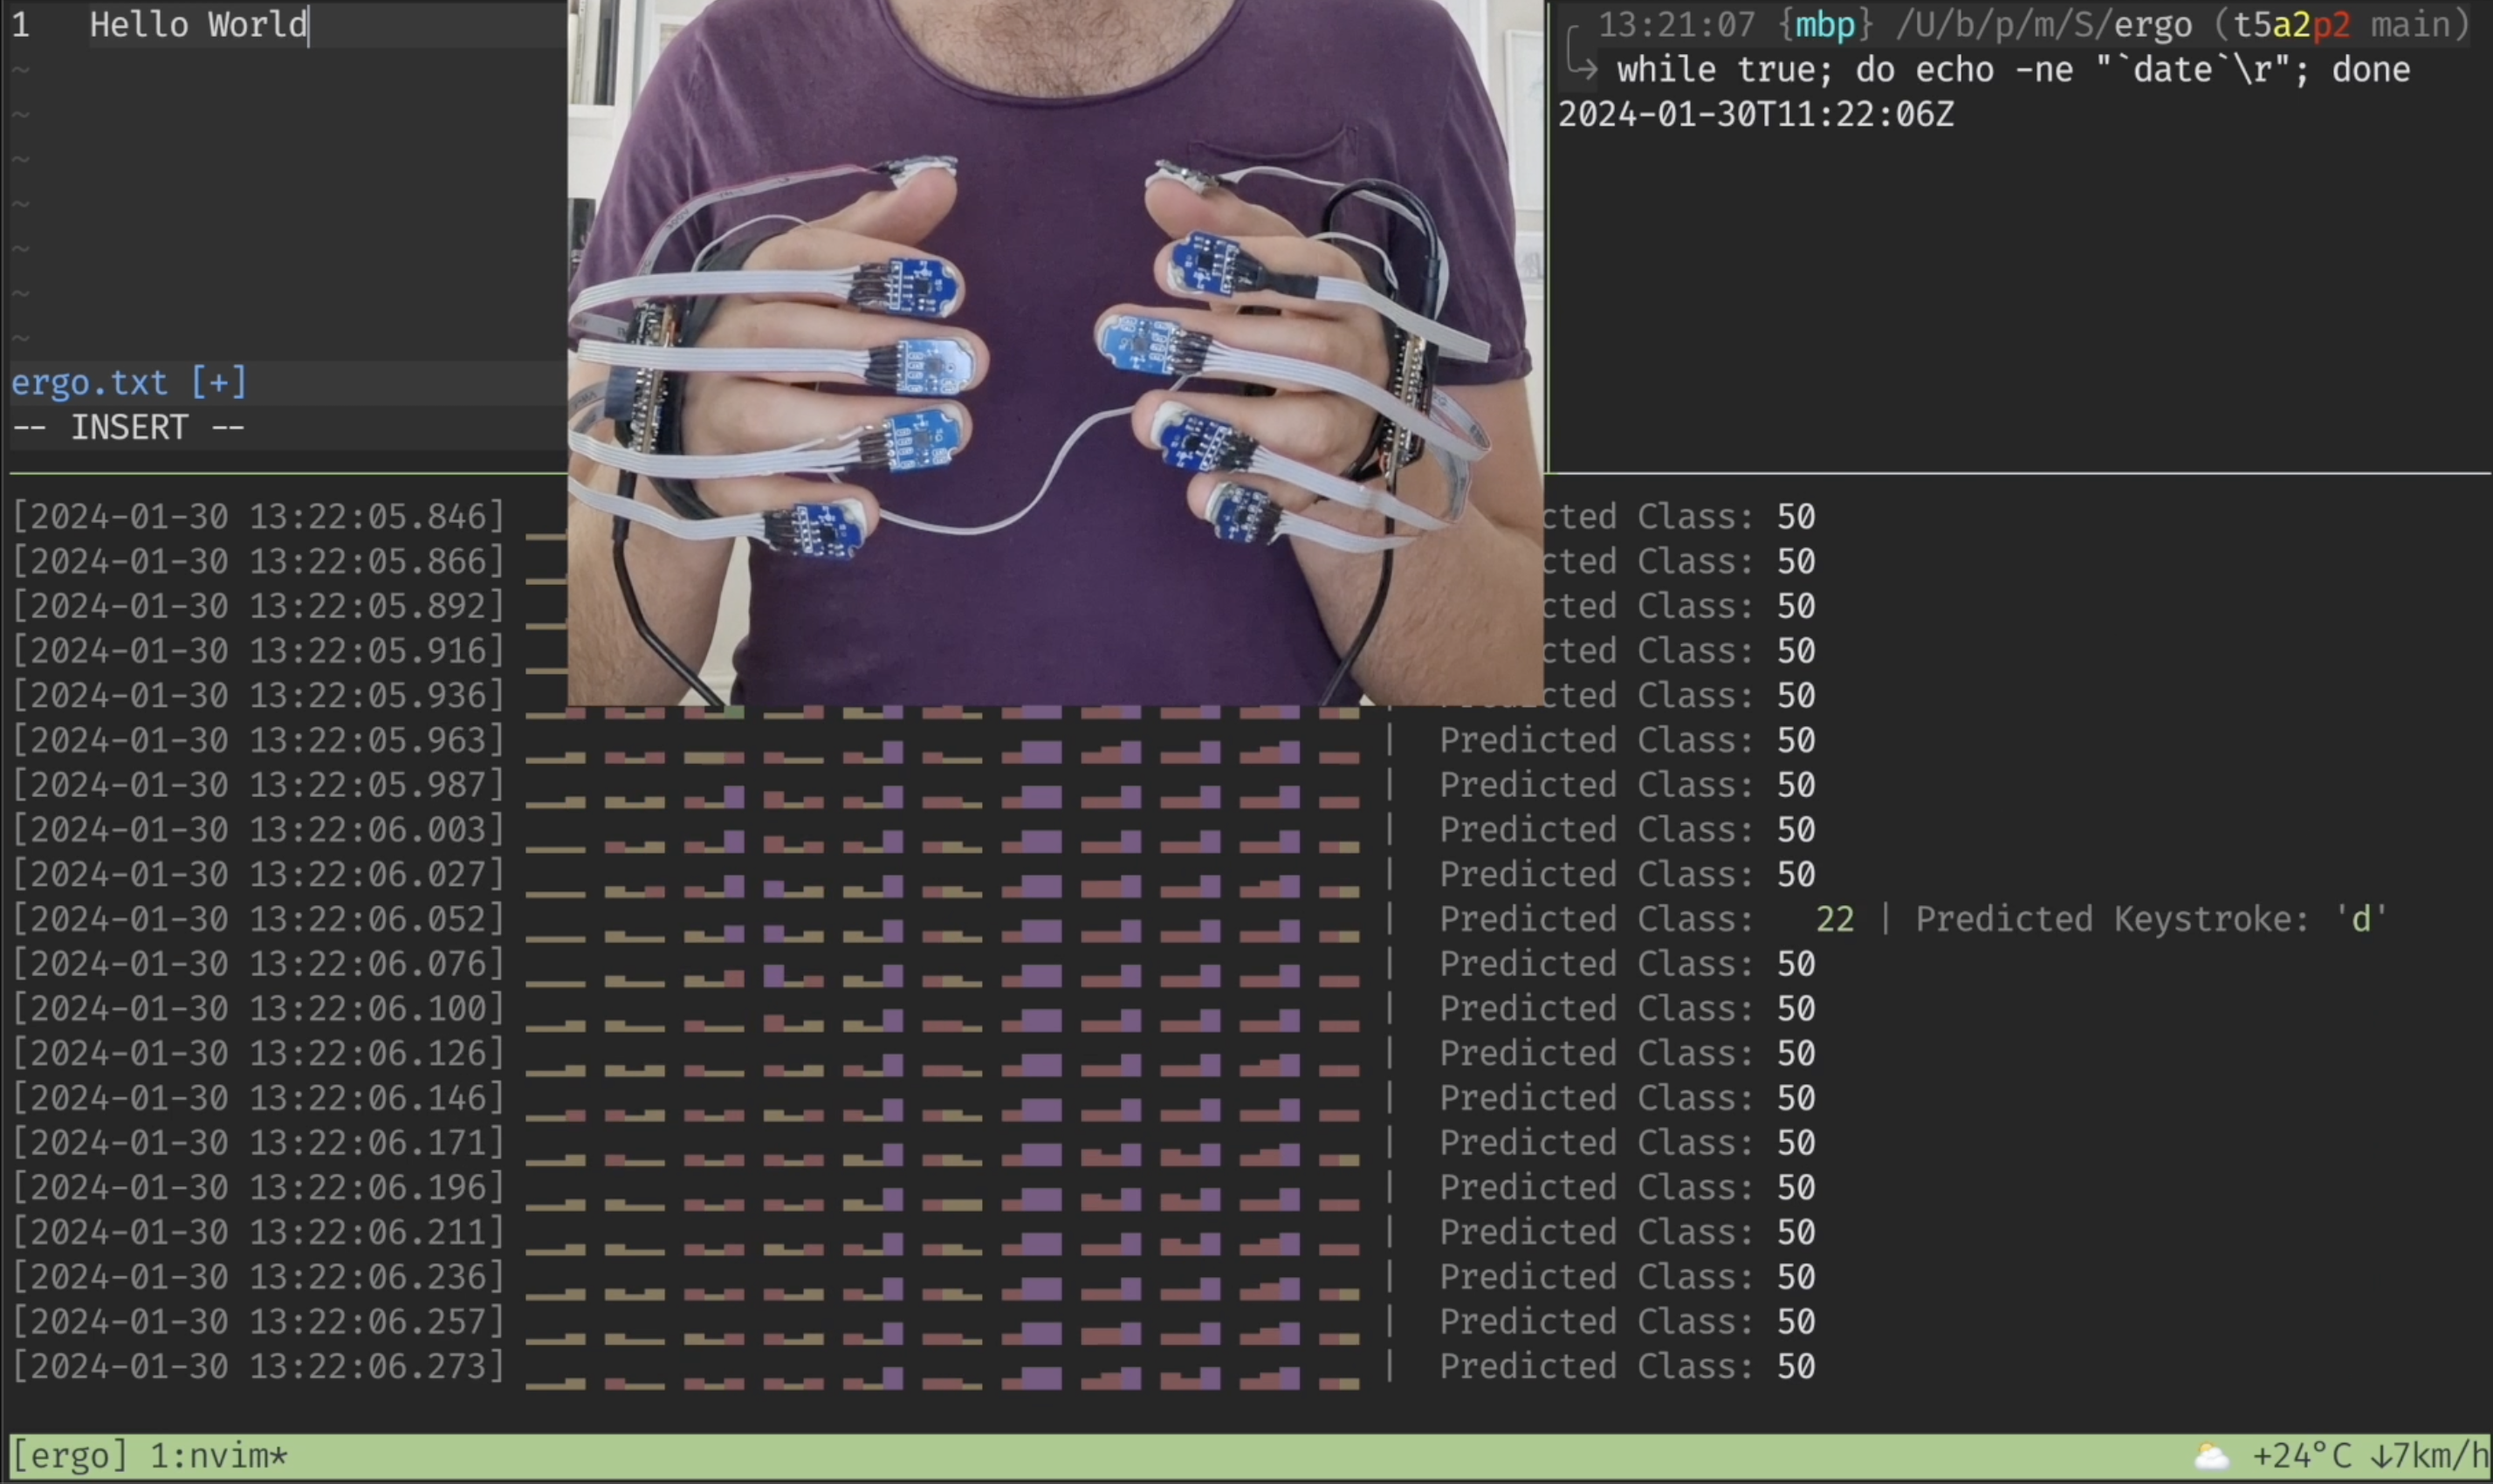
\includegraphics[width=0.9\textwidth]{video_thumbnail.png}
    \end{figure}
    \emph{Ergo} in a nutshell:
    \begin{enumerate}
        \item Similar to a glove in form-factor
        \item Sensors measure fingertip acceleration
        \item Acceleration measurements are classified into gestures
        \item Gestures are mapped to keystrokes
        \item Keystrokes are sent to the operating system
    \end{enumerate}
\end{frame}

\section{Introduction}
\begin{frame}
    \frametitle{Introduction}
    \framesubtitle{Research questions}
    \centering
    1. Evaluate hardware performance
\end{frame}

\begin{frame}
    \frametitle{Introduction}
    \framesubtitle{Research questions}
    \centering
    2. Compare algorithm performance
\end{frame}

\begin{frame}
    \frametitle{Introduction}
    \framesubtitle{Research questions}
    \centering
    3. Extract gestures from background noise
\end{frame}

\begin{frame}
    \frametitle{Introduction}
    \framesubtitle{Research questions}
    \centering
    4. Assess impact of noise on performance
\end{frame}

\begin{frame}
    \frametitle{Introduction}
    \framesubtitle{Research questions}
    \centering
    5. Assess classification speed
\end{frame}

\begin{frame}
    \frametitle{Introduction}
    \framesubtitle{Open Code, Open Data}
    \begin{itemize}
        \item All code is on
            GitHub\footnote{https://github.com/beyarkay/masters‐code}.
        \item The source code for the thesis (and this presentation) is also on
            GitHub\footnote{https://github.com/beyarkay/masters‐thesis}.
        \item The dataset is on
            Zenodo\footnote{https://zenodo.org/records/10209419}.
        \item The video played at the beginning of the presentation is
            available on
            YouTube\footnote{https://www.youtube.com/watch?v=vFsaH1TqNWo}.
    \end{itemize}
\end{frame}

\section{Background}
\begin{frame}
    \frametitle{Background}
    \framesubtitle{Models and Algorithms}
    \begin{columns}
        \begin{column}{.5\textwidth}
            \begin{figure}
            
\includegraphics[height=0.2\textheight, width=\linewidth, keepaspectratio]{todo}
                \caption{Feed-Forward Neural Networks (FFNNs)}
            \end{figure}
        \end{column}
        \begin{column}{.5\textwidth}
            \begin{figure}
            
\includegraphics[height=0.2\textheight, width=\linewidth, keepaspectratio]{todo}
                \caption{Support Vector Machines (SVMs)}
            \end{figure}
        \end{column}
    \end{columns}
    \begin{columns}
        \begin{column}{.5\textwidth}
            \begin{figure}
            
\includegraphics[height=0.2\textheight, width=\linewidth, keepaspectratio]{todo}
                \caption{Hidden Markov Models (HMMs)}
            \end{figure}
        \end{column}
        \begin{column}{.5\textwidth}
            \begin{figure}
            
\includegraphics[height=0.2\textheight, width=\linewidth, keepaspectratio]{todo}
                \caption{Cumulative Sum (CuSUM)}
            \end{figure}
        \end{column}
    \end{columns}
\end{frame}

\begin{frame}
    \frametitle{Background}
    \framesubtitle{$F_1$-score, confusion matrices, and evaluation metrics}
    todo
\end{frame}

\section{Literature Review}
\begin{frame}
    \frametitle{Literature Review}
    \framesubtitle{Seminal work}
    something something sturman, animac
\end{frame}

\begin{frame}
    \frametitle{Literature Review}
    \framesubtitle{Technologies Used Over Time}
    plot goes here
\end{frame}

\begin{frame}
    \frametitle{Literature Review}
    \framesubtitle{Number of Classes Over Time}
    plot goes here
\end{frame}

\begin{frame}
    \frametitle{Literature Review}
    \framesubtitle{Algorithms Used Over Time}
    plot goes here
\end{frame}

\begin{frame}
    \frametitle{Literature Review}
    \framesubtitle{Gesture Fidelity Over Time}
    plot goes here
\end{frame}

\begin{frame}
    \frametitle{Literature Review}
    \framesubtitle{Explicit/Implicit Segmentation Over Time}
    plot goes here
\end{frame}

\section{Methodology}
\begin{frame}
    \frametitle{Methodology}
    \begin{columns}[T] % T aligns the tops of the columns
    \begin{column}{0.5\textwidth}
        \begin{itemize}
            \item \emph{Ergo} is built with two Arduino Nano 33 BLEs, two
                CD74HC4067 multiplexers, and ten ADXL335 accelerometers.
        \end{itemize}
    \end{column}
    \begin{column}{0.5\textwidth}
        % Your image here
        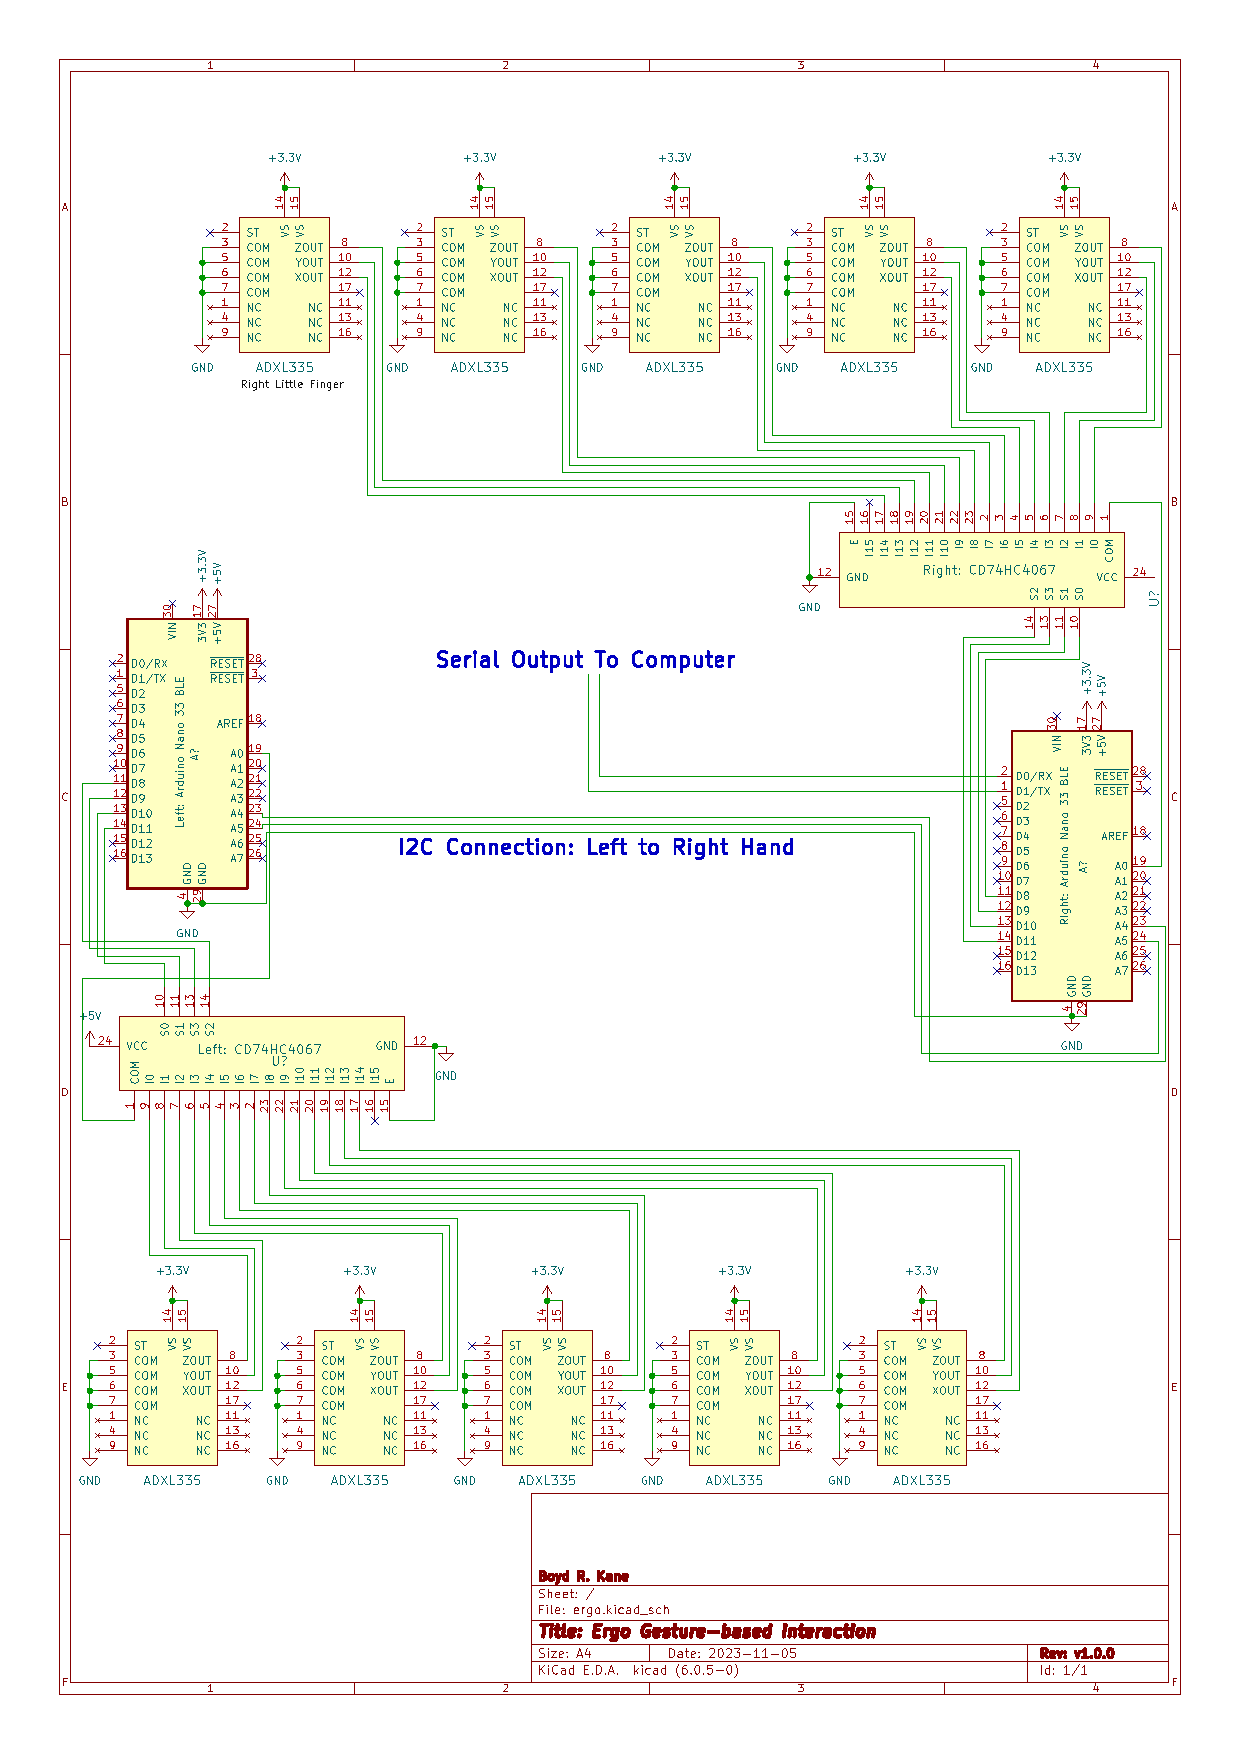
\includegraphics[width=\textwidth]{ergo_schematic.pdf}
    \end{column}
    \end{columns}
\end{frame}

\begin{frame}
    \begin{itemize}
        \item Gestures are converted to keystrokes using a simple mapping
    \end{itemize}
    \begin{figure}[h]
        \centering
        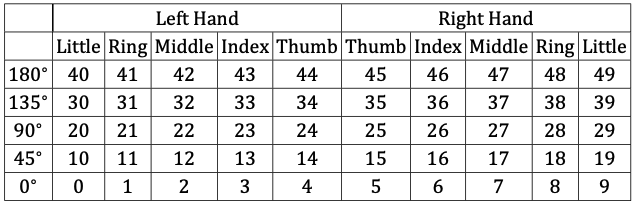
\includegraphics[width=0.9\textwidth]{mapping_idxs.png}
        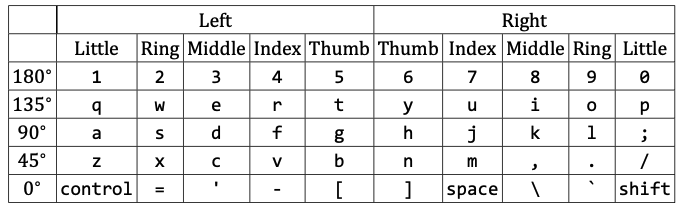
\includegraphics[width=0.9\textwidth]{mapping_qwerty.png}
    \end{figure}
\end{frame}


\section{Results}
\begin{frame}
    \frametitle{Results}
    \begin{itemize}
        \item HMMs \& CuSUM failed to learn the data
        \item SVM performed well
        \item FFNNs and HFFNNs performed well, but with many failure states
    \end{itemize}
    % Your image here
    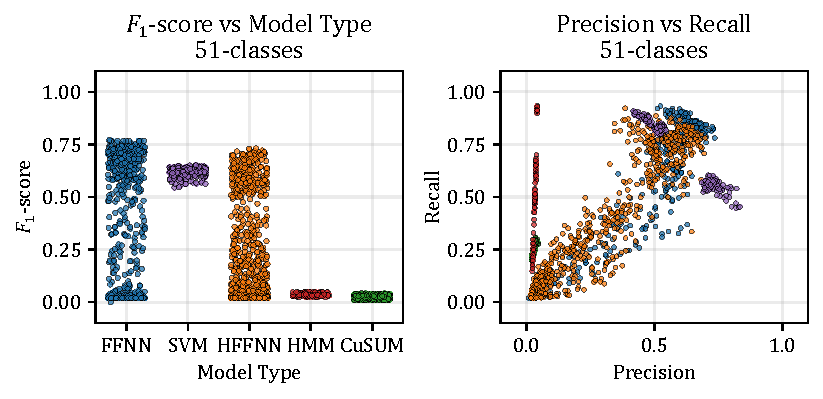
\includegraphics[width=\textwidth]{05_precision_recall_51_classes.pdf}
\end{frame}

\begin{frame}
    On the unseen test set, the best performing model (an FFNN) performs well.
    % Your image here
    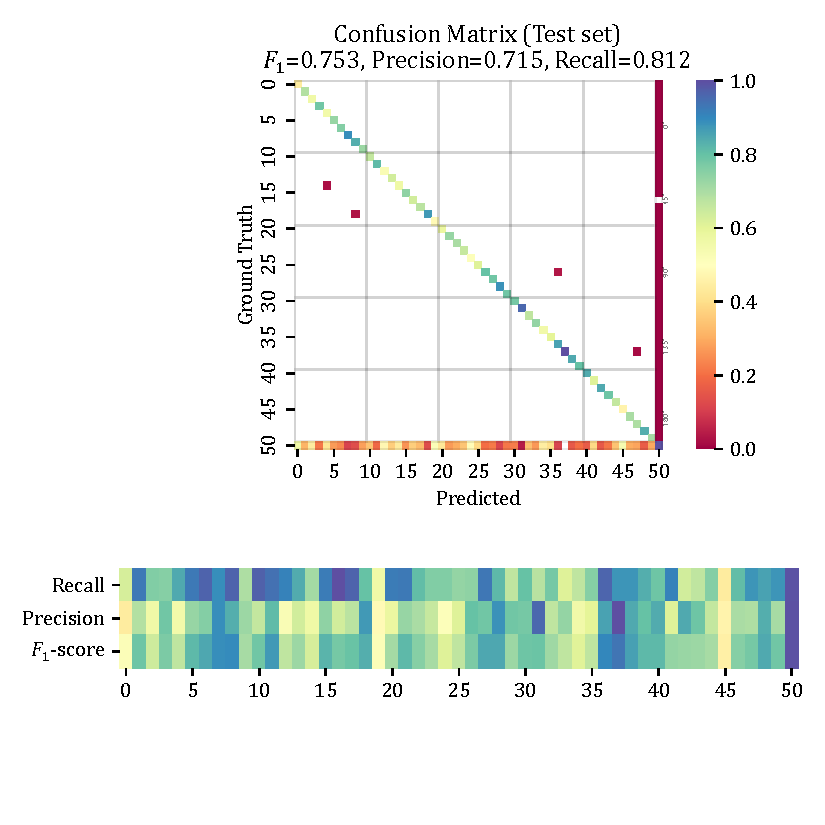
\includegraphics[width=\textwidth]{05_tst_set_conf_mat.pdf}
\end{frame}

\begin{frame}
    \texttt{the quick brown fox jumped over the lazy dog}
    \begin{figure}[h]
        \centering
        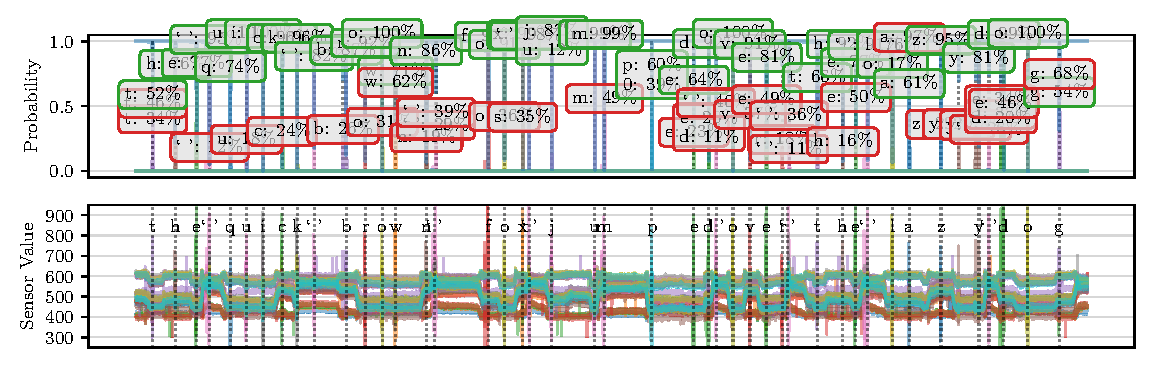
\includegraphics[width=\textwidth]{05_pred_plot_0000_to_9420_full_text.pdf}
    \end{figure}
\end{frame}

\begin{frame}
    \begin{figure}[h]
        \centering
        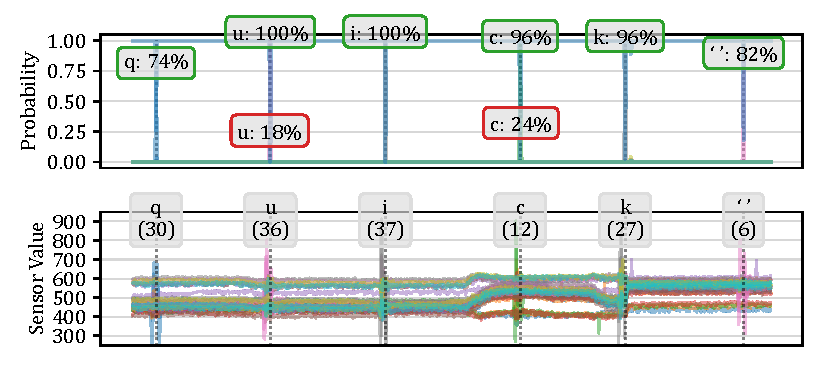
\includegraphics[width=\textwidth]{05_pred_plot_0900_to_1800_quick.pdf}
    \end{figure}
\end{frame}

\section{Conclusion}
\begin{frame}
    \frametitle{Conclusion}
    Research Questions:
    \begin{enumerate}
        \item Evaluate hardware performance
        \item Compare algorithm performance
        \item Extract gestures from background noise
        \item Assess impact of noise on performance
        \item Assess classification speed
    \end{enumerate}
\end{frame}

\end{document}
